\section{Investigación sobre Oracle}

Desde su versión 8i, el motor de base de datos \texttt{Oracle} utiliza tres buffer pools para tener bloques de datos. Un resumen sucinto de la arquitectura de buffers
en \texttt{Oracle} puede verse en la figura \ref{fotito}.

\begin{figure}[H]\centering
	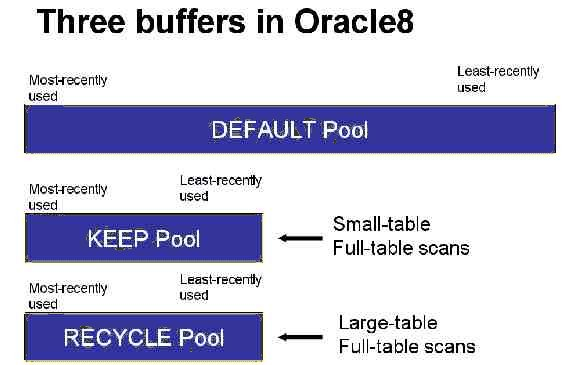
\includegraphics[scale=0.5]{keepRecycle.jpg}
	\caption{Los tres buffers de \texttt{Oracle 8i}}
	\label{fotito}
\end{figure}
\subsection{Uso}
Para utilizar los distintos buffer pools, se marcan objetos de la base de datos de tal forma que quedan asociados a un pool particular. Luego de esto, todos los bloques asociados a ese objeto (un bloque no puede tener elementos de distintos objetos) irá siempre a ese buffer\footnote{http://docs.oracle.com/cd/B10500\_01/server.920/a96533/memory.htm}. 

Es digno observar que estos buffers no tienen un comportamiento automático. Es el usuario quien debe encargarse de marcar qué páginas irán a qué buffer para que los buffers acá definidos sean utilizados. 

\subsubsection{Ejemplo}
\begin{Verbatim}[xleftmargin=-3em]
	CREATE TABLE t1 (
		my_date   DATE NOT NULL,
		my_number NUMBER(12,10) NOT NULL,
		my_row    NUMBER(12) NOT NULL)
	STORAGE (BUFFER_POOL KEEP);	
\end{Verbatim}

\subsection{Default pool}
Es el espacio de memoria que se utiliza por defecto para los bloques que pertenecen a objetos que no fueron marcados específicamente para ser usados con otras tablas.

\subsection{Keep pool}
El buffer \texttt{keep} se usa para tablas e índices que son utilizados muy frecuentemente. El uso habitual de este pool de memoria es mantener bloques que son frecuentemente accedidos. 

Este buffer pool es particularmente eficiente a la hora de ``proteger'' a los bloques de memoria más frecuentemente utilizados de los nocivos efectos de desalojo masivo que tienen las implementaciones más triviales de \textit{full table scan}. Generalmente, al realizar una de estas consultas se requiere mucha memoria, lo que termina forzando que un gran número de bloques de tablas frecuentemente utilizadas sean desartadas y sea necesario volver a traerlos de disco si se quieren volver a utilizar. Es por esto que \texttt{Oracle} permite marcar tablas para que estas vayan al buffer \texttt{keep}. De esta forma se intenta evitar su pérdida cuando deben ser desalojados por alguna query.

Notar que este método no es 100\% efectivo, dado que muy probablemente la suma de los bloques de todas las tablas marcadas como \texttt{keep} (así sea una sola) supere el tamaño del buffer. Con lo cual en algún momento es posible que sea necesario guardar un bloque en el buffer \texttt{keep} cuando este esté lleno, con lo que va a tener que descartarse algún bloque mediante alguna política de reemplazo (en \texttt{Oracle}, generalmente \textit{LRU}). 

En general se recomienda que el buffer \texttt{keep} sea utilizado para objetos pequeños \footnote{http://www.exploreoracle.com/2009/04/02/keep-buffer-pool-and-recycle-buffer-pool/}.

\subsection{Recycle pool}
A diferencia del \texttt{keep} buffer, el \texttt{recycle} buffer debe ser utilizado con bloques pertenecientes a tablas que son raramente accedidos. Los bloques que están en este pool son descartados rápidamente una vez que dejan de ser utilizados \footnotemark[\value{footnote}]. Esto es porque en Oracle existe una opción \textit{ASM} que, usada en este caso, permite realocar la memoria del \texttt{recycle} a otro componente del SGA (\textit{System Global Area}, un componente que forma parte del sistema de administración de memoria del DMBS).

Por recomendación de \texttt{Oracle}\footnote{http://docs.oracle.com/cd/B28359\_01/server.111/b28274/memory.htm\#autoId29}, el tamaño del \texttt{recycle} pool debe ser lo suficientemente chico como para no ocupar RAM que podría ser mejor destinada a otro pool (como lo bloques se desalojan relativamente rápido, es mucho mejor usado el espacio en el default o \texttt{keep} pool), pero lo suficientemente grande como para que un bloque no sea desalojado en medio de una transacción (supongamos una transacción que levanta un bloque de un objeto marcado de \texttt{recycle}, luego lo procesa junto con otros y luego lo escribe. Si el \texttt{recycle} buffer es demasiado pequeño y fue necesario desalojar el bloque durante el procesado, a la hora de grabarlo va a ser necesario volver a levantarlo, lo que es mucho más ineficiente).

Históricamente (en \texttt{Oracle 8}), el \texttt{recycle} pool comenzó como un buffer donde alojar bloques \textit{transitorios}\footnote{http://www.praetoriate.com/t\_\%20tuning\_recycle\_pool.htm}. Un bloque \textit{transitorio} es aquel que se lee como parte de un \textit{full table scan} y es poco probable que vuelva a ser utilizado en el futuro cercano. Este concepto luego fue extendido de bloques transitorios a cualquier bloque perteneciente a objetos particulares que el dba sepa que serán utilizados muy esparsamente.